\documentclass{article}
\usepackage[utf8]{inputenc}
\usepackage[legalpaper, margin=1in]{geometry}

\usepackage[english]{babel}

\usepackage{amsmath}
\usepackage{amssymb}
\usepackage{amsthm}
\usepackage{physics}

\usepackage{graphicx}

\usepackage{xcolor}
\usepackage{listings}
\usepackage{makecell}

\usepackage{hyperref}
\usepackage{cleveref}

\usepackage{marginnote}
\usepackage{csquotes}
\usepackage{todonotes}

\usepackage{listings}
\usepackage{xcolor}
\definecolor{codegreen}{rgb}{0,0.6,0}
\definecolor{codegray}{rgb}{0.5,0.5,0.5}
\definecolor{codepurple}{rgb}{0.58,0,0.82}
\definecolor{backcolour}{rgb}{0.95,0.95,0.92}
\lstdefinestyle{mystyle}{
    backgroundcolor=\color{backcolour},   
    commentstyle=\color{codegreen},
    keywordstyle=\color{magenta},
    numberstyle=\tiny\color{codegray},
    stringstyle=\color{codepurple},
    basicstyle=\ttfamily\footnotesize,
    breakatwhitespace=false,         
    breaklines=true,                 
    captionpos=b,                    
    keepspaces=true,                 
    numbers=left,                    
    numbersep=5pt,                  
    showspaces=false,                
    showstringspaces=false,
    showtabs=false,                  
    tabsize=2
}
\lstset{style=mystyle}

\newtheorem{definition}{Definition}
\newtheorem{theorem}{Theorem}
\newtheorem{lemma}{Lemma}
\newtheorem{corollary}[lemma]{Corollary}
\newtheorem{property}{Property}

\title{CSC2516: Programming Assignment 2: Convolutional Neural Networks}
\author{}
\date{February 2021}

\begin{document}

\maketitle

\section*{Part A: Pooling and Upsampling}

\subsection*{1 Complete the model \texttt{PoolUpsampleNet}}

\begin{lstlisting}[language=Python]
#V202102171018
class PoolUpsampleNet(nn.Module):
    def __init__(self, kernel, num_filters, num_colours, num_in_channels):
        super().__init__()

        # Useful parameters
        padding = kernel // 2

        ############### YOUR CODE GOES HERE ############### 
        # Input: [BS, NIC, 32, 32]
        self.block0 = nn.Sequential(
            nn.Conv2d(in_channels=num_in_channels, 
                      out_channels=num_filters, 
                      kernel_size=kernel, 
                      padding=padding),
            nn.MaxPool2d(kernel_size=2),
            nn.BatchNorm2d(num_features=num_filters),
            nn.ReLU()
        )
        # Output: [BS, NF, 16, 16]
        self.block1 = nn.Sequential(
            nn.Conv2d(in_channels=num_filters, 
                      out_channels=2*num_filters, 
                      kernel_size=kernel, 
                      padding=padding),
            nn.MaxPool2d(kernel_size=2),
            nn.BatchNorm2d(num_features=2*num_filters),
            nn.ReLU()
        )
        # Output: [BS, 2NF, 8, 8]
        self.block2 = nn.Sequential(
            nn.Conv2d(in_channels=2*num_filters, 
                      out_channels=num_filters, 
                      kernel_size=kernel, 
                      padding=padding),
            nn.Upsample(scale_factor=2),
            nn.BatchNorm2d(num_features=num_filters),
            nn.ReLU()
        )
        # Output: [BS, NF, 16, 16]
        self.block3 = nn.Sequential(
            nn.Conv2d(in_channels=num_filters, 
                      out_channels=num_colours, 
                      kernel_size=kernel, 
                      padding=padding),
            nn.Upsample(scale_factor=2),
            nn.BatchNorm2d(num_features=num_colours),
            nn.ReLU()
        )
        # Output: [BS, NC, 32, 32]
        self.block4 = nn.Sequential(
            nn.Conv2d(in_channels=num_colours, 
                      out_channels=num_colours, 
                      kernel_size=kernel, 
                      padding=padding)
        )
        # Output: [BS, NC, 32, 32]
        ###################################################

    def forward(self, x):
        ############### YOUR CODE GOES HERE ###############
        for block in (self.block0, self.block1, self.block2, 
                      self.block3, self.block4):
            x = block.forward(x)
        return x
        ###################################################
\end{lstlisting}

\subsection*{2 Run main training loop of \texttt{PoolUpsampleNet}}

\begin{lstlisting}[language=Python]
...
Epoch [25/25], Loss: 1.5852, Time (s): 33
Epoch [25/25], Val Loss: 1.5785, Val Acc: 41.6%, Time(s): 34.18
\end{lstlisting}

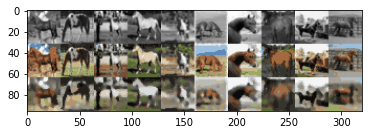
\includegraphics{A2.1.png}

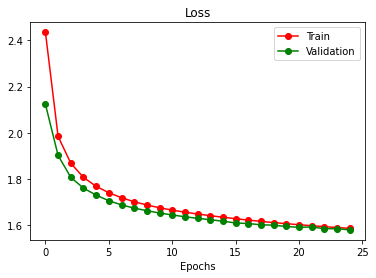
\includegraphics{A2.2.png}

\begin{quote}
Do these results look good to you?  Why or why not?
\end{quote}

The images appear blurry because in the network they were up-sampled from 8x8 back to 32x32. The background and saddles also appear poorly coloured.

\subsection*{3 Compute the number of weights, outputs, and connections in the model}

\todo{Check Piazza}






\section*{Part B: Strided and Transposed Convolutions}

\subsection*{1 Complete the model \texttt{ConvTransposeNet}}

\begin{lstlisting}[language=Python]
#V202102171234
class ConvTransposeNet(nn.Module):
    def __init__(self, kernel, num_filters, num_colours, num_in_channels):
        super().__init__()

        # Useful parameters
        stride = 2
        padding = kernel // 2
        output_padding = 1

        ############### YOUR CODE GOES HERE ############### 
        # Input: [BS, NIC, 32, 32]
        self.block0 = nn.Sequential(
            nn.Conv2d(in_channels=num_in_channels, 
                      out_channels=num_filters, 
                      kernel_size=kernel, 
                      padding=padding,
                      stride=stride),
            nn.BatchNorm2d(num_features=num_filters),
            nn.ReLU()
        )
        # Output: [BS, NF, 16, 16]
        self.block1 = nn.Sequential(
            nn.Conv2d(in_channels=num_filters, 
                      out_channels=2*num_filters, 
                      kernel_size=kernel, 
                      padding=padding,
                      stride=stride),
            nn.BatchNorm2d(num_features=2*num_filters),
            nn.ReLU()
        )
        # Output: [BS, 2NF, 8, 8]
        self.block2 = nn.Sequential(
            nn.ConvTranspose2d(in_channels=2*num_filters, 
                      out_channels=num_filters, 
                      kernel_size=kernel, 
                      padding=padding,
                      output_padding=output_padding,
                      stride=stride),
            nn.BatchNorm2d(num_features=num_filters),
            nn.ReLU()
        )
        # Output: [BS, NF, 16, 16]
        self.block3 = nn.Sequential(
            nn.ConvTranspose2d(in_channels=num_filters, 
                      out_channels=num_colours, 
                      kernel_size=kernel, 
                      padding=padding,
                      output_padding=output_padding,
                      stride=stride),
            nn.BatchNorm2d(num_features=num_colours),
            nn.ReLU()
        )
        # Output: [BS, NC, 32, 32]
        self.block4 = nn.Sequential(
            nn.Conv2d(in_channels=num_colours, 
                      out_channels=num_colours, 
                      kernel_size=kernel, 
                      padding=padding)
        )
        # Output: [BS, NC, 32, 32]
        ###################################################

    def forward(self, x):
        ############### YOUR CODE GOES HERE ###############
        for block in (self.block0, self.block1, self.block2, 
                      self.block3, self.block4):
            x = block.forward(x)
        return x
        ###################################################
\end{lstlisting}

\subsection*{Train the model}


\begin{lstlisting}[language=Python]
...
Epoch [25/25], Loss: 1.2070, Time (s): 104
Epoch [25/25], Val Loss: 1.1603, Val Acc: 54.7%, Time(s): 105.78
\end{lstlisting}

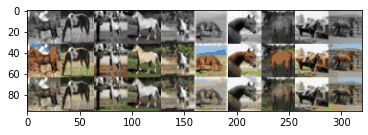
\includegraphics{B2.1.png}

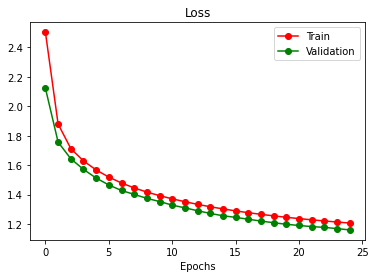
\includegraphics{B2.2.png}


\subsection*{3 How do the result compare to Part A?}

The result qualitatively appear similar as before. The current \texttt{ConvTransposeNet} model seems to be worse at colouring brown horses.

The current model resulted in \emph{lower} validation loss (1.2) compared to the previous model (1.6). The \texttt{ConvTranspose2d} layers produce lower loss than \texttt{Upsample} because the transposed convolutions fits additional weights to ``reverse'' the previous skipping done by the convolution, resulting in a better numeric fitting and lower loss. 


\subsection*{4 \texttt{padding} parameter}

\begin{tabular}{ c c c }
	 & \texttt{nn.Conv2d}  & \texttt{nn.ConvTranspose2d} \\ 
	 \hline
	if kernel size = 4 & \texttt{padding}=1 & \makecell{\texttt{padding}=1 \\ \texttt{output\_padding}=0} \\  
	if kernel size = 5 & \texttt{padding}=2 & \makecell{\texttt{padding}=2 \\ \texttt{output\_padding}=1}
\end{tabular}
%\todo{verify}


\subsection*{5 Describe  the  effect  of  batch  sizes  on  the  training/validation loss, and the final image output quality.}

Smaller batch sizes were associated with lower training/validation loss and the output quality was better with smaller batch sizes. 



\section{Part C: Skip Connections}

\subsection*{1 Add a skip connection...}

\begin{lstlisting}[language=Python]
	#V202102200047
	class UNet(nn.Module):
	    def __init__(self, kernel, num_filters, num_colours, num_in_channels):
	        super().__init__()
	
	        # Useful parameters
	        stride = 2
	        padding = kernel // 2
	        output_padding = 1
	
	        ############### YOUR CODE GOES HERE ############### 
	        # Input: [BS, NIC, 32, 32]
	        self.block0 = nn.Sequential(
	            nn.Conv2d(in_channels=num_in_channels, 
	                      out_channels=num_filters, 
	                      kernel_size=kernel, 
	                      padding=padding),
	            nn.MaxPool2d(kernel_size=2),
	            nn.BatchNorm2d(num_features=num_filters),
	            nn.ReLU()
	        )
	        # Output: [BS, NF, 16, 16]
	        self.block1 = nn.Sequential(
	            nn.Conv2d(in_channels=num_filters, 
	                      out_channels=2*num_filters, 
	                      kernel_size=kernel, 
	                      padding=padding),
	            nn.MaxPool2d(kernel_size=2),
	            nn.BatchNorm2d(num_features=2*num_filters),
	            nn.ReLU()
	        )
	        # Output: [BS, 2NF, 8, 8]
	        self.block2 = nn.Sequential(
	            nn.Conv2d(in_channels=2*num_filters, 
	                      out_channels=num_filters, 
	                      kernel_size=kernel, 
	                      padding=padding),
	            nn.Upsample(scale_factor=2),
	            nn.BatchNorm2d(num_features=num_filters),
	            nn.ReLU()
	        )
	        # Concatenate
	        # Output: [BS, NF+NF, 16, 16]
	        self.block3 = nn.Sequential(
	            nn.Conv2d(in_channels=num_filters+num_filters, 
	                      out_channels=num_colours, 
	                      kernel_size=kernel, 
	                      padding=padding),
	            nn.Upsample(scale_factor=2),
	            nn.BatchNorm2d(num_features=num_colours),
	            nn.ReLU()
	        )
	        # Concatenate
	        # Output: [BS, NC+NIC, 32, 32]
	        self.block4 = nn.Sequential(
	            nn.Conv2d(in_channels=num_colours+num_in_channels, 
	                      out_channels=num_colours, 
	                      kernel_size=kernel, 
	                      padding=padding)
	        )
	        # Output: [BS, NC, 32, 32]
	        ###################################################
	
	    def forward(self, x):
	        ############### YOUR CODE GOES HERE ###############
	        x_input = x
	        x = self.block0(x)
	        x_1 = x
	        x = self.block1(x)
	        x = self.block2(x)
	        x = torch.cat((x_1, x), dim=1)
	        x = self.block3(x)
	        x = torch.cat((x_input, x), dim=1)
	        x = self.block4(x)
	        return x
	        ###################################################
\end{lstlisting}

\subsection*{Train the model}


\begin{lstlisting}[language=Python]
	...
	Epoch [25/25], Loss: 1.3075, Time (s): 33
	Epoch [25/25], Val Loss: 1.3323, Val Acc: 48.2%, Time(s): 34.52
\end{lstlisting}

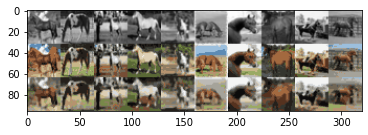
\includegraphics{C2.1.png}

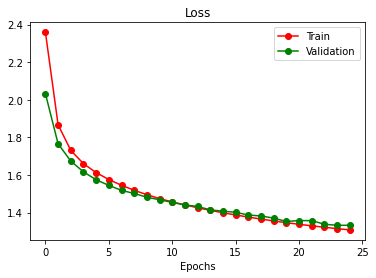
\includegraphics{C2.2.png}

\subsection*{ How  does  the  result  compare  to  the  previous  mode}

The skip connections did not improve validation loss as compared to the previous model, but improved the output qualitatively. The brown horses were coloured closer to the actual brown colour. The improvements come from:

\begin{enumerate}
\item The skip connections allows high resolution, low level features that did not need convolution operation or only one convolution to be directly passed down to the final layers. 
\item More channels in the final two layers increased the complexity and parameters of the model.
\end{enumerate}


















\end{document}
